% questions.tex —— 2002 年·全国新课程卷·文科 · 题目内容片段（无答案）
% 由 tools/generate_projects.py 依来源总账自 2002/2002_数学真题_全国新课程文_试题.md 生成，勿手改（改源 MD 后重跑）


\gkpart{数学}

\begin{gktip}
\textbf{来源说明}：本题面依据固定源 PDF 两页 A3 题面逐题转录，原卷印刷页码 116–117。固定源不附答案，答案和解析均由本库独立复算。

\textbf{图形说明}：第 13 题和第 19 题的原卷图形关系重绘为 TikZ/PGFPlots 矢量图。图形标记所指的 PNG 不随仓库保存。
\end{gktip}

\gkpart{一、选择题}

\begin{question}
\gkti{1}直线 $(1+a)x+y+1=0$ 与圆 $x^2+y^2-2x=0$ 相切，则 $a$ 的值为\mbox{（　　）}

（A）$\pm1$　　（B）$\pm2$　　（C）$1$　　（D）$-1$

\end{question}
\begin{question}
\gkti{2}已知 $m\text{、}n$ 为异面直线，$m\subset$ 平面 $\alpha$，$n\subset$ 平面 $\beta$，$\alpha\cap\beta=l$，则 $l$\mbox{（　　）}

（A）与 $m\text{、}n$ 都相交

（B）与 $m\text{、}n$ 中至少一条相交

（C）与 $m\text{、}n$ 都不相交

（D）至多与 $m\text{、}n$ 中的一条相交

\end{question}
\begin{question}
\gkti{3}函数 $y=a^x$ 在 $[0,1]$ 上的最大值与最小值之和为 $3$，则 $a=$\mbox{（　　）}

（A）$\dfrac12$　　（B）$2$　　（C）$4$　　（D）$\dfrac14$

\end{question}
\begin{question}
\gkti{4}不等式 $(1+x)(1-|x|)>0$ 的解集是\mbox{（　　）}

（A）$\{x\mid 0\leqslant x<1\}$

（B）$\{x\mid x<0\text{ \text{且} }x\neq-1\}$

（C）$\{x\mid -1<x<1\}$

（D）$\{x\mid x<1\text{ \text{且} }x\neq-1\}$

\end{question}
\begin{question}
\gkti{5}在 $(0,2\pi)$ 内，使 $\sin x>\cos x$ 成立的 $x$ 的取值范围是\mbox{（　　）}

（A）$\left(\dfrac\pi4,\dfrac\pi2\right)\cup\left(\pi,\dfrac{5\pi}4\right)$

（B）$\left(\dfrac\pi4,\pi\right)$

（C）$\left(\dfrac\pi4,\dfrac{5\pi}4\right)$

（D）$\left(\dfrac\pi4,\pi\right)\cup\left(\dfrac{5\pi}4,\dfrac{3\pi}2\right)$

\end{question}
\begin{question}
\gkti{6}设集合

\nopagebreak[4]
\[
M=\left\{x\middle|x=\frac{k}{2}+\frac14,\ k\in\mathbb Z\right\},\qquad
N=\left\{x\middle|x=\frac{k}{4}+\frac12,\ k\in\mathbb Z\right\},
\]

则\mbox{（　　）}

（A）$M=N$　　（B）$M\subseteq N$　　（C）$M\supseteq N$　　（D）$M\cap N=\varnothing$

\end{question}
\begin{question}
\gkti{7}椭圆 $5x^2+ky^2=5$ 的一个焦点是 $(0,2)$，那么 $k=$\mbox{（　　）}

（A）$-1$　　（B）$1$　　（C）$\sqrt5$　　（D）$-\sqrt5$

\end{question}
\begin{question}
\gkti{8}正六棱柱 $ABCDEF-A_1B_1C_1D_1E_1F_1$ 的底面边长为 $1$，侧棱长为 $\sqrt2$，则这个棱柱侧面对角线 $E_1D$ 与 $BC_1$ 所成的角是\mbox{（　　）}

（A）$90^\circ$　　（B）$60^\circ$　　（C）$45^\circ$　　（D）$30^\circ$

\end{question}
\begin{question}
\gkti{9}函数 $y=x^2+bx+c$，$x\in[0,+\infty)$ 是单调函数的充要条件是\mbox{（　　）}

（A）$b\geqslant0$　　（B）$b\leqslant0$　　（C）$b>0$　　（D）$b<0$

\end{question}
\begin{question}
\gkti{10}已知 $0<x<y<a<1$，则有\mbox{（　　）}

（A）$\log_a(xy)<0$

（B）$0<\log_a(xy)<1$

（C）$1<\log_a(xy)<2$

（D）$\log_a(xy)>2$

\end{question}
\begin{question}
\gkti{11}从正方体的 6 个面中选取 3 个面，其中有 2 个面不相邻的选法共有\mbox{（　　）}

（A）8 种　　（B）12 种　　（C）16 种　　（D）20 种

\end{question}
\begin{question}
\gkti{12}平面直角坐标系中，$O$ 为坐标原点，已知两点 $A(3,1)\text{、}B(-1,3)$，若点 $C$ 满足

\nopagebreak[4]
\[
\overrightarrow{OC}=\alpha\overrightarrow{OA}+\beta\overrightarrow{OB},
\qquad \alpha,\beta\in\mathbb R,\quad \alpha+\beta=1,
\]

则点 $C$ 的轨迹方程为\mbox{（　　）}

（A）$3x+2y-11=0$

（B）$(x-1)^2+(y-2)^2=5$

（C）$2x-y=0$

（D）$x+2y-5=0$

\end{question}
\gkpart{二、填空题}

\Needspace{0.4\textheight}
\begin{question}
\gkti{13}据新华社 2002 年 3 月 12 日电，1985 年到 2000 年间，我国农村人均居住面积如图所示，其中，从\gkblank{}年到\gkblank{}年的五年间增长最快。
\nopagebreak[4]
\begin{center}% 2002 年全国新课程文科第 13 题：农村人均居住面积折线图
\begin{tikzpicture}[x=0.9cm,y=0.25cm,>=stealth]
  \draw[->] (0,0)--(10.5,0) node[right] {年份};
  \draw[->] (0,0)--(0,31) node[above] {面积/$\mathrm{m^2}$};
  \foreach \y/\label in {10/10,15/15,20/20,25/25,30/30}
    \draw (-0.12,\y)--(0.12,\y) node[left=5pt] {\label};
  \foreach \x/\label in {1/1985,4/1990,7/1995,10/2000}
    \draw (\x,0.15)--(\x,-0.15) node[below=4pt] {\label};
  \draw[thick] (1,14.7)--(4,17.8)--(7,21.0)--(10,24.8);
  \foreach \x/\y/\label in {
    1/14.7/14.7,
    4/17.8/17.8,
    7/21.0/21.0,
    10/24.8/24.8}
  {
    \fill (\x,\y) circle (1.4pt);
    \node[above=3pt] at (\x,\y) {\label};
  }
\end{tikzpicture}
\end{center}
\nopagebreak[4]
\begin{center}
\begin{tabular}{lrrrr}
\toprule
年份 & 1985 & 1990 & 1995 & 2000 \\
\midrule
人均居住面积（$\mathrm{m^2}$） & 14.7 & 17.8 & 21.0 & 24.8 \\
\bottomrule
\end{tabular}
\end{center}

\end{question}
\begin{question}
\gkti{14}已知 $\sin2\alpha=-\sin\alpha$，$\alpha\in\left(\dfrac\pi2,\pi\right)$，则 $\cot\alpha=$\gkblank{}。

\end{question}
\begin{question}
\gkti{15}甲、乙两种冬小麦试验品种连续 5 年的平均单位面积产量如下（单位：$\mathrm{t/km^2}$）：

\begin{center}
\begin{tabular}{lrrrrr}
\toprule
品种 & 第 1 年 & 第 2 年 & 第 3 年 & 第 4 年 & 第 5 年 \\
\midrule
甲 & 9.8 & 9.9 & 10.1 & 10.0 & 10.2 \\
乙 & 9.4 & 10.3 & 10.8 & 9.7 & 9.8 \\
\bottomrule
\end{tabular}
\end{center}

其中产量比较稳定的小麦品种是\gkblank{}。

\end{question}
\begin{question}
\gkti{16}设函数 $f(x)$ 在 $(-\infty,+\infty)$ 内有定义，下列函数

① $y=-|f(x)|$；② $y=xf(x^2)$；③ $y=-f(-x)$；④ $y=f(x)-f(-x)$。

其中必为奇函数的有\gkblank{}。（要求填写正确答案的序号）

\end{question}
\gkpart{三、解答题}

\begin{question}
\gkti{17}在等比数列 $\{a_n\}$ 中，已知 $a_6-a_4=24$，$a_3a_5=64$，求 $\{a_n\}$ 前 8 项的和 $S_8$。

\end{question}
\begin{question}
\gkti{18}已知 $\sin^2 2\alpha+\sin2\alpha\cos\alpha-\cos2\alpha=1$，$\alpha\in\left(0,\dfrac\pi2\right)$，求 $\sin\alpha\text{、}\tan\alpha$ 的值。

\Needspace{0.4\textheight}
\end{question}
\begin{question}
\gkti{19}【甲】正三棱柱 $ABC-A_1B_1C_1$ 的底面边长为 $a$，侧棱长为 $\sqrt2a$。
\nopagebreak[4]
\begin{center}% 2002 年全国新课程文科第 19 题甲：正三棱柱
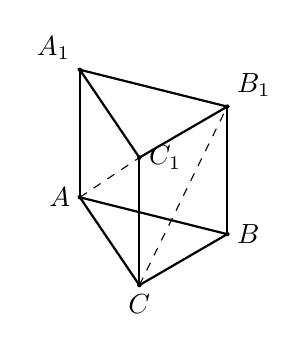
\begin{tikzpicture}[>=stealth,scale=0.72]
  \coordinate (A) at (0,0);
  \coordinate (B) at (2.6,-0.65);
  \coordinate (C) at (1.05,-1.55);
  \coordinate (Aone) at (0,2.25);
  \coordinate (Bone) at (2.6,1.60);
  \coordinate (Cone) at (1.05,0.70);
  \draw[thick] (A)--(B)--(C)--cycle;
  \draw[thick] (Aone)--(Bone)--(Cone)--cycle;
  \draw[thick] (A)--(Aone) (B)--(Bone) (C)--(Cone);
  \draw[dashed] (A)--(Cone) (C)--(Bone);
  \fill (A) circle (1.1pt) node[left] {$A$};
  \fill (B) circle (1.1pt) node[right] {$B$};
  \fill (C) circle (1.1pt) node[below] {$C$};
  \fill (Aone) circle (1.1pt) node[above left] {$A_1$};
  \fill (Bone) circle (1.1pt) node[above right] {$B_1$};
  \fill (Cone) circle (1.1pt) node[right] {$C_1$};
\end{tikzpicture}
\end{center}
\nopagebreak[4]
（1） 建立适当的坐标系，并写出点 $A\text{、}B\text{、}A_1\text{、}C_1$ 的坐标；

（2） 求 $AC_1$ 与侧面 $ABB_1A_1$ 所成的角。

【乙】如图，正方形 $ABCD\text{、}ABEF$ 的边长都是 1，而且平面 $ABCD\text{、}ABEF$ 互相垂直。点 $M$ 在 $AC$ 上移动，点 $N$ 在 $BF$ 上移动，若 $CM=BN=a$（$0<a<\sqrt2$）。
\nopagebreak[4]
\begin{center}% 2002 年全国新课程文科第 19 题乙：两个互相垂直的正方形
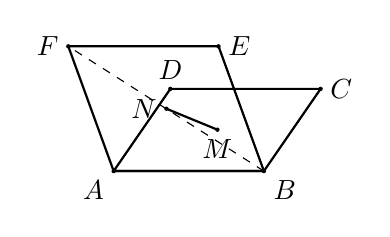
\begin{tikzpicture}[>=stealth,scale=0.72]
  \coordinate (A) at (0,0);
  \coordinate (B) at (2.65,0);
  \coordinate (C) at (3.65,1.45);
  \coordinate (D) at (1.0,1.45);
  \coordinate (E) at (1.85,2.20);
  \coordinate (F) at (-0.80,2.20);
  \coordinate (M) at (1.83,0.73);
  \coordinate (N) at (0.93,1.10);
  \draw[thick] (A)--(B)--(C)--(D)--cycle;
  \draw[thick] (A)--(B)--(E)--(F)--cycle;
  \draw[dashed] (A)--(D) (B)--(F);
  \draw[thick] (M)--(N);
  \fill (A) circle (1.1pt) node[below left] {$A$};
  \fill (B) circle (1.1pt) node[below right] {$B$};
  \fill (C) circle (1.1pt) node[right] {$C$};
  \fill (D) circle (1.1pt) node[above] {$D$};
  \fill (E) circle (1.1pt) node[right] {$E$};
  \fill (F) circle (1.1pt) node[left] {$F$};
  \fill (M) circle (1.1pt) node[below] {$M$};
  \fill (N) circle (1.1pt) node[left] {$N$};
\end{tikzpicture}
\end{center}
\nopagebreak[4]
（1） 求 $MN$ 的长；

（2） $a$ 为何值时，$MN$ 的长最小；

（3） 当 $MN$ 的长最小时，求面 $MNA$ 与面 $MNB$ 所成二面角 $\alpha$ 的大小。

\end{question}
\begin{question}
\gkti{20}某单位 6 个员工借助互联网开展工作，每个员工上网的概率都是 0.5（相互独立）。

（1） 求至少 3 人同时上网的概率；

（2） 至少几人同时上网的概率小于 0.3？

\end{question}
\begin{question}
\gkti{21}已知 $a>0$，函数 $f(x)=x^3-a$，$x\in(0,+\infty)$。设 $x_1>0$，记曲线 $y=f(x)$ 在点 $(x_1,f(x_1))$ 处的切线为 $l$。

（1） 求 $l$ 的方程；

（2） 设 $l$ 与 $x$ 轴交点为 $(x_2,0)$。证明：

① $x_2\geqslant\sqrt[3]{a}$；

② 若 $x_2>\sqrt[3]{a}$，则 $\sqrt[3]{a}<x_2<x_1$。

\end{question}
\begin{question}
\gkti{22}已知两点 $M(-1,0)\text{、}N(1,0)$，且点 $P$ 使 $\overrightarrow{MP}\cdot\overrightarrow{MN}$、$\overrightarrow{PM}\cdot\overrightarrow{PN}$、$\overrightarrow{NM}\cdot\overrightarrow{NP}$ 成公差小于零的等差数列。

（1） 点 $P$ 的轨迹是什么曲线？

（2） 若点 $P$ 坐标为 $(x_0,y_0)$，记 $\theta$ 为 $\overrightarrow{PM}$ 与 $\overrightarrow{PN}$ 的夹角，求 $\tan\theta$。

\end{question}